\documentclass[conference]{IEEEtran}
\IEEEoverridecommandlockouts

\DeclareRobustCommand{\IEEEauthorrefmark}[1]{\smash{\textsuperscript{\footnotesize #1}}}

\usepackage{cite}
\usepackage{amsmath,amssymb,amsfonts}
\usepackage{graphicx}
\usepackage{booktabs}
\usepackage[hidelinks]{hyperref}
\usepackage{xcolor}
\usepackage{tikz}

\def\BibTeX{{\rm B\kern-.05em{\sc i\kern-.025em b}\kern-.08em
    T\kern-.1667em\lower.7ex\hbox{E}\kern-.125emX}}

% -------------------- Notation helpers --------------------
\newcommand{\Tsw}{T_{\mathrm{sw}}}
\newcommand{\tsamp}{t_{\mathrm{samp}}}
\newcommand{\tacq}{t_{\mathrm{acq}}}
\newcommand{\tconv}{t_{\mathrm{conv}}}
\newcommand{\tbusy}{t_{\mathrm{busy}}}
\newcommand{\tblank}{t_{\mathrm{blank}}}
\newcommand{\tmargin}{t_{\mathrm{margin}}}
\newcommand{\treq}{t_{\mathrm{req}}}
\newcommand{\midx}{m}
\newcommand{\dc}{d}

\begin{document}

\title{Acquisition-Time Limited Modulation in Single-Shunt Current Reconstruction for PMSM FOC}

\author{
    \IEEEauthorblockN{
        Mark Wendler\IEEEauthorrefmark{1},
        and J\'ozsef Kopj\'ak\IEEEauthorrefmark{2}
    }
    \IEEEauthorblockA{
        \IEEEauthorrefmark{1}Doctoral School of Applied Informatics and Applied Mathematics,
        {\'O}buda University, Budapest, Hungary\\
        Email: mark.wendler@phd.uni-obuda.hu
    }
    \IEEEauthorblockA{
        \IEEEauthorrefmark{2}Kand\'o K\'alm\'an Faculty of Electrical Engineering,
        {\'O}buda University, Budapest, Hungary\\
        Email: kopjak.jozsef@kvk.uni-obuda.hu
    }
}

\maketitle

\begin{abstract}
Single-shunt (DC-link) current sensing is a popular low-cost option for field-oriented control (FOC) of permanent-magnet synchronous motors (PMSM), but its feasibility is dictated by pulse-width-modulation (PWM) geometry: two accurate analog-to-digital converter (ADC) samples must be captured inside two active-vector plateaus of every PWM cycle. This paper reframes the ADC requirement from headline ``mega-samples-per-second'' (MSPS) to a \emph{settling-driven acquisition time}, and derives a compact, closed-form relationship between the required per-sample window and the maximum achievable modulation index (and duty cycle) under center-aligned space-vector modulation (SVM). We distinguish two operating regimes---unmodified PWM, which leaves blind zones near sector boundaries, and minimum-window enforcement, which guarantees full-angle reconstruction at the cost of modulation headroom---and show that in both cases the binding parameter is the analog acquisition/settling budget, not converter throughput. The result yields a direct design rule connecting analog front-end settling, blanking, and trigger margin to usable voltage headroom, and clarifies why single-shunt sensing is uniquely sensitive to the analog signal chain and to silicon-integration limits of on-chip amplifiers.
\end{abstract}

\begin{IEEEkeywords}
PMSM, FOC, single shunt, DC-link current sensing, SVM, ADC acquisition time, modulation index
\end{IEEEkeywords}

% -------------------- Section I --------------------
\section{Scope and Contributions}
FOC of a PMSM relies on precise stator-current feedback that is time-aligned to the PWM carrier \cite{Krause2013,Krishnan2010}. In \emph{sensorless} operation, current-measurement error feeds the observer/PLL and re-emerges as electrical-angle error, increasing torque ripple and copper loss \cite{Vas1998,Holtz2002}. In cost-sensitive embedded drives, single-shunt sensing is attractive but imposes the tightest timing constraints, because all three phase currents must be reconstructed from samples of a single DC-link current captured during limited SVM plateaus \cite{Blaabjerg1997,Bose2002}.



In a companion analysis of dual- and three-shunt timing we showed that, once the system effective number of bits (ENOB) is adequate, the dominant accuracy constraint is whether the analog chain \emph{settles inside} the valid PWM window, and that for dual-shunt sensing the settling budget imposes only an \emph{upper} modulation bound \cite{wendler_enhancing_2025,wendler_analysis_2025}. This paper completes that program for the single-shunt case.

\textbf{Contributions:}
\begin{itemize}
\item a concise topology and integration overview explaining why sensorless control magnifies the impact of current-sensing error;
\item a timing-first ADC requirement for single-shunt sensing, where, unlike multi-shunt sensing, conversion time can become co-limiting because two samples share one channel;
\item the main result: a closed-form link between the ADC acquisition-time budget and the maximum modulation index (and duty) for full-angle single-shunt reconstruction under center-aligned SVM, together with the blind-zone description for unmodified PWM;
\item a discussion of mitigation strategies and of how external versus integrated analog front ends---and the silicon node on which they are built---set the achievable settling time.
\end{itemize}

% -------------------- Section II --------------------
\section{Shunt Topologies and Integration Context}
Simplified schematics on figure~\ref{fig:3phase_current_topologies} and table~\ref{tab:topologies} summarizes four common shunt placements used with three-phase inverters \cite{Krause2013,Bose2002,Kester2005}.

\begin{figure}
    \centering
    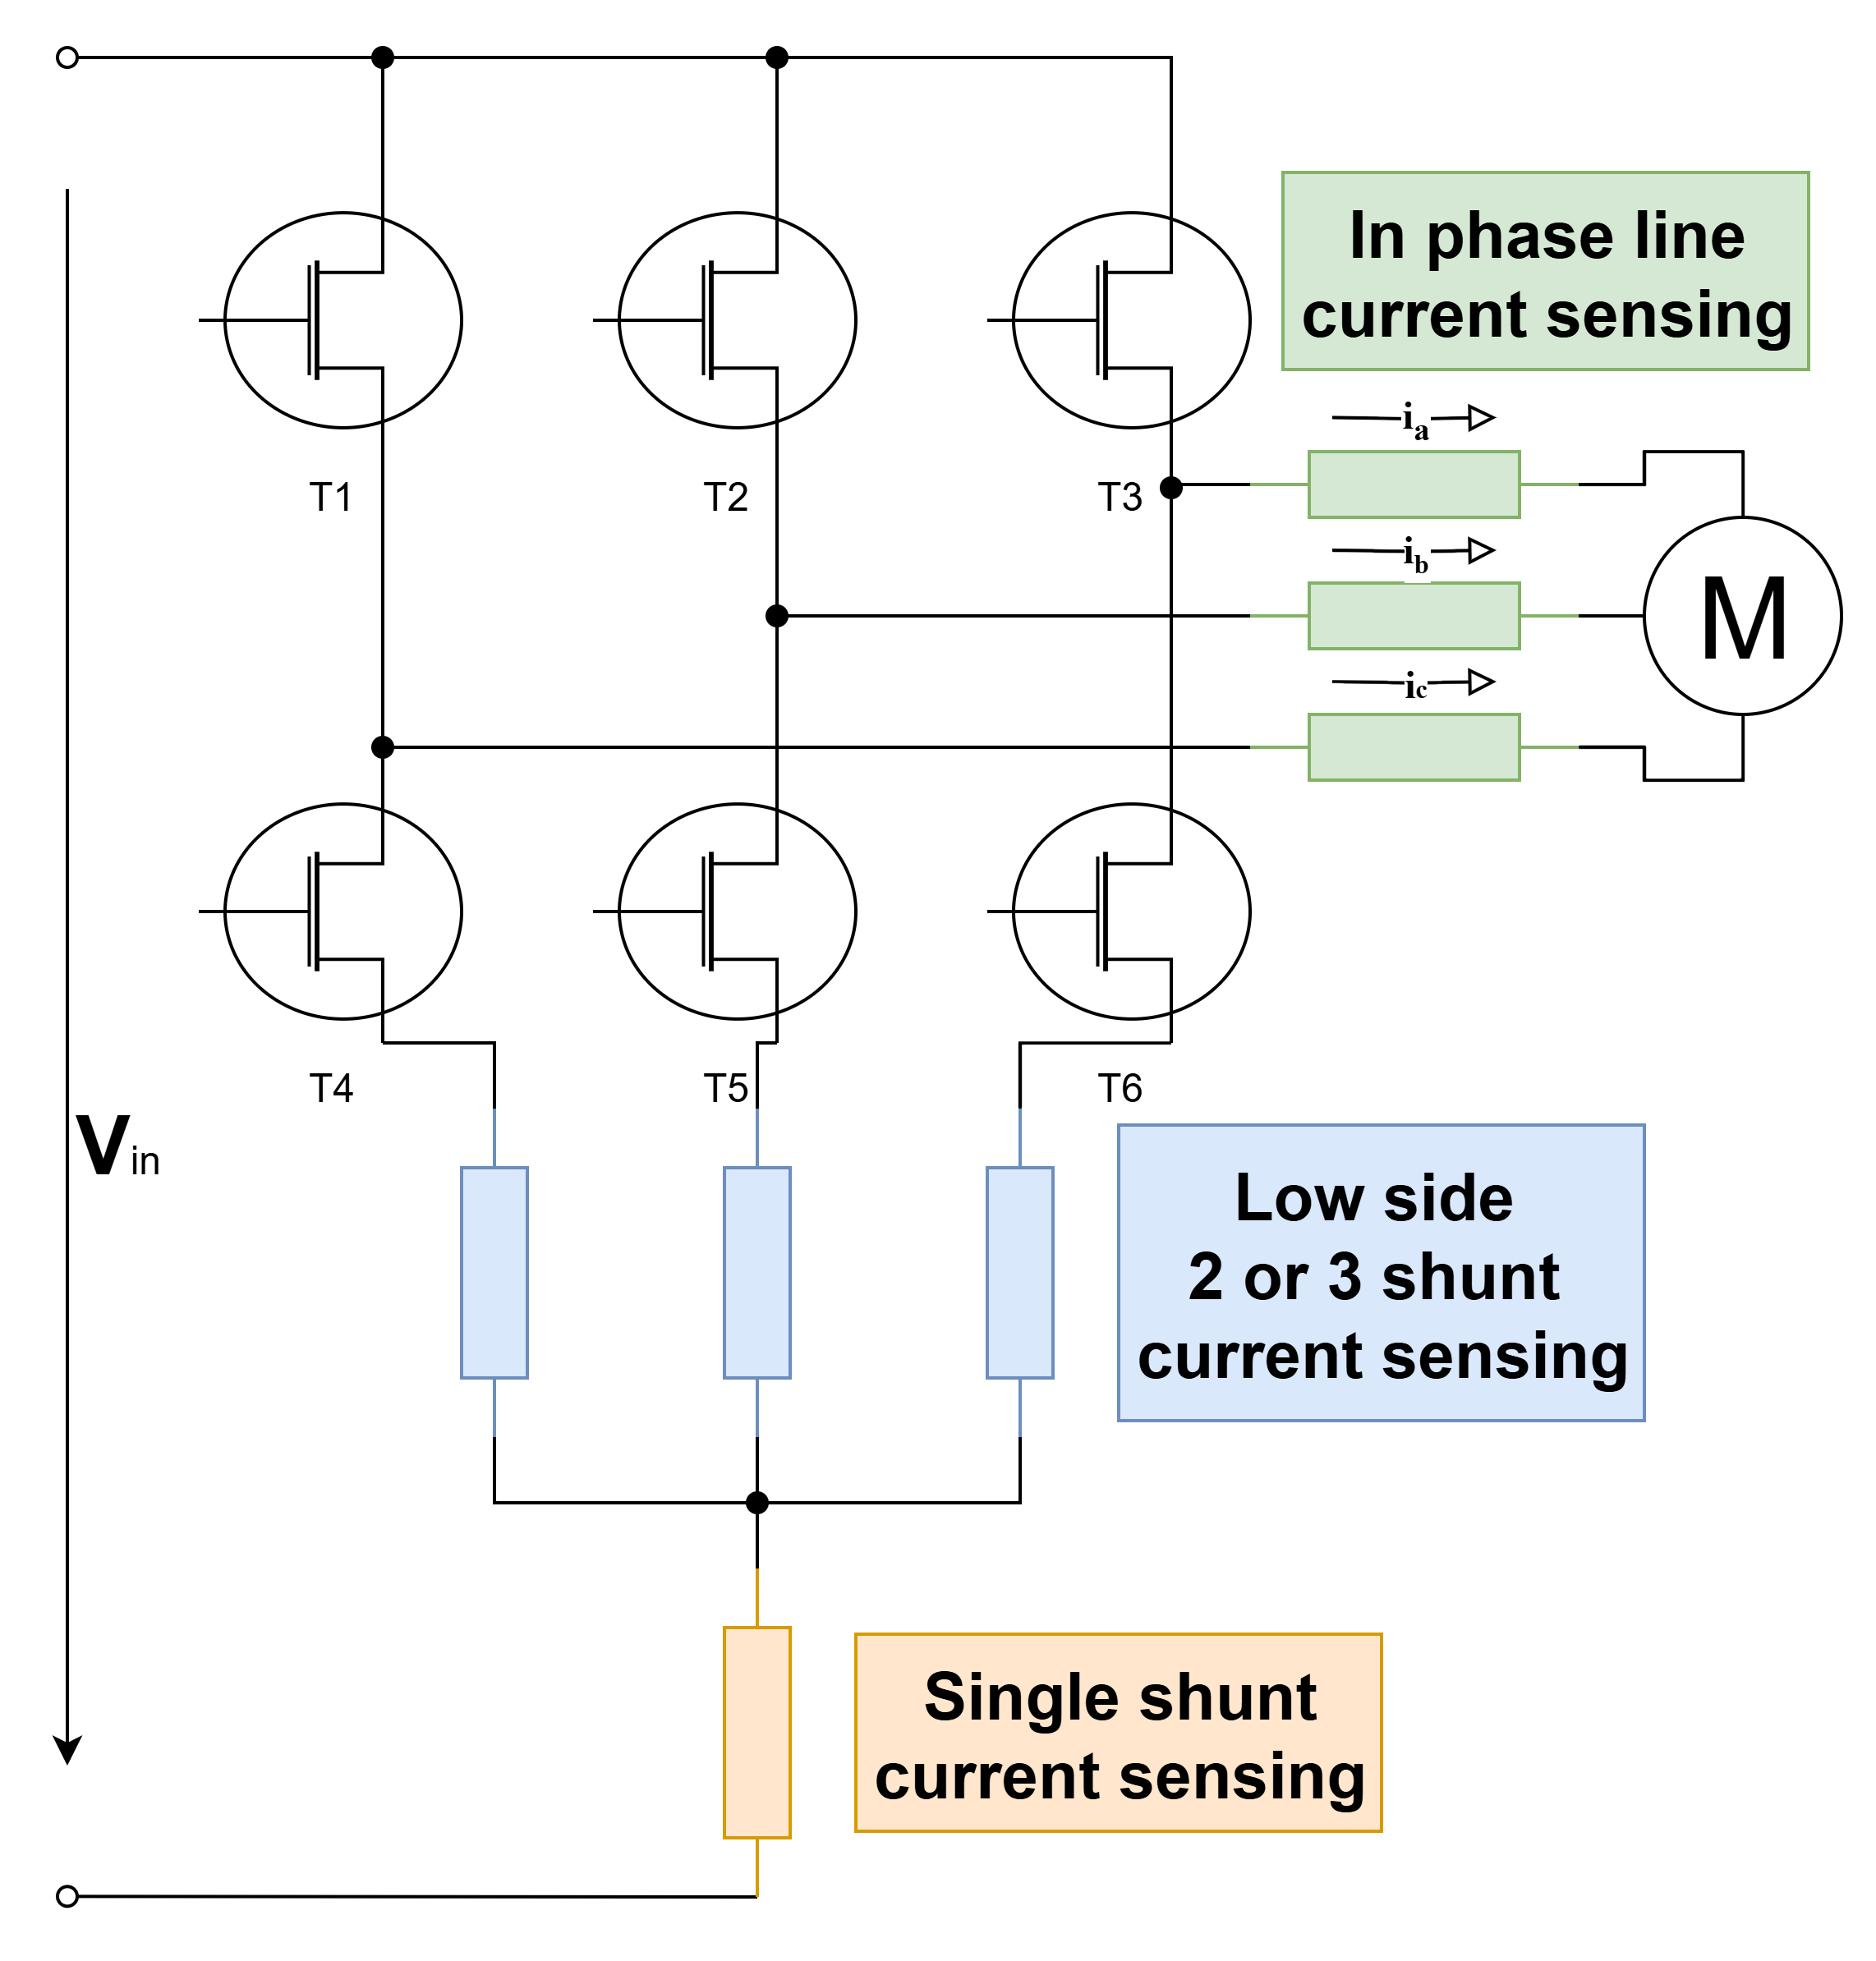
\includegraphics[width=1\linewidth]{Drawings/CurrentMeasWithCurrentLabel.png}
    \caption{3-phase Current sensing topologies}
    \label{fig:3phase_current_topologies}
\end{figure}

\begin{table}[t]
\caption{Shunt topologies: qualitative trade-offs}
\label{tab:topologies}
\centering
\begin{tabular}{@{}p{2.05cm}p{2.7cm}p{2.7cm}@{}}
\toprule
\textbf{Topology} & \textbf{Strengths} & \textbf{Constraints} \\
\midrule
In-line phase shunts &
Direct phase currents, simplest reconstruction, best SNR potential, sampling freedom (oversampling) &
Common-mode stress, isolation often needed at high bus voltage \\
\addlinespace
Low-side 3-shunt &
Direct currents (low CM), robust timing &
More components and ADC channels \\
\addlinespace
Low-side 2-shunt &
Lower cost than 3-shunt, reconstruction via $i_a{+}i_b{+}i_c{=}0$ &
Timing skew and reconstruction sensitivity \\
\addlinespace
Low-side single shunt (DC-link) &
Lowest cost and smallest footprint, single channel &
Two samples must fit SVM plateaus; blind zones near sector edges \\
\bottomrule
\end{tabular}
\end{table}

\noindent\textbf{Voltage and integration context.}
At higher bus voltages, typical of mains-fed appliance drives ($>100$~V), in-line sensing usually demands galvanic or capacitive isolation and careful handling of fast common-mode edges, which adds cost and propagation delay. At lower bus voltages, typical of battery-operated products ($<100$~V), low-side sensing with integrated programmable-gain amplifiers (PGA) or op-amps is common and economical. However, integrated front ends are themselves a timing bottleneck: their common-mode step response and finite gain-bandwidth consume part of the sampling window. This pressure is intensifying as motor-control MCUs migrate to advanced digital nodes (e.g., sub-$40$~nm), where high-performance analog---low-offset amplifiers, fast gate drivers, precision references---does not scale as favorably as logic, so on-chip front ends often trade settling time and noise for integration and cost. Single-shunt sensing, which depends on \emph{two} fast settled samples per period, is the topology most exposed to this trade-off.

% -------------------- Section III --------------------
\section{Precision Challenge: Sensorless vs.\ Sensored}
\subsection{Why sensorless often needs cleaner current measurement}
For surface-PM machines with $i_d\!\approx\!0$, torque is proportional to $i_q$ \cite{Krause2013}. In sensorless control, current error perturbs the observer model and produces an electrical-angle error $\Delta\theta$, effectively rotating the $dq$ frame. To hold torque, the controller must raise $|i_q|$ by $1/\cos\Delta\theta$; since copper loss scales with current squared, a small-angle expansion gives
\begin{equation}
\frac{\Delta P_{\mathrm{cu}}}{P_{\mathrm{cu}}} \approx \frac{1}{\cos^2\Delta\theta}-1 \approx \Delta\theta^2 \qquad (\Delta\theta \text{ in rad}),
\label{eq:cu_loss}
\end{equation}
so even modest RMS angle error measurably increases loss and reduces efficiency \cite{Holtz2002,Vas1998}. In sensored control (encoder/resolver) the angle is measured, so the same current error is \emph{not} amplified by an additional angle-estimation path. Engineering takeaway: for the same efficiency target, sensorless FOC typically demands tighter current-measurement quality---offset, noise, and, crucially, timing-induced error \cite{kofler_sensorless_2025}.

\subsection{ADC ``bits'' are necessary but not sufficient}
Resolution/ENOB sets a baseline noise floor, but in a PWM environment the dominant failure mode is \emph{sampling the wrong value} because the analog front end has not settled after a switching transition. For shunt sensing, the limiting parameter is therefore not headline MSPS but the time required to acquire a settled sample inside the available plateau \cite{Kester2005}. Throughput-centric selection metrics \cite{ADI_EE365_2013,NXP_AN4608_2012,MathWorks_MCB_Sampling_2025,TI_SLAAE96A_2023,ST_AN3116_2010,Microchip_AN1078_2010} are necessary for picking the loop-update rate and DMA bandwidth, but secondary for instantaneous fidelity.

% -------------------- Section IV --------------------
\section{Timing Model: Acquisition Time Inside the PWM Window}
We adopt the physical requirement that a sample is valid only if the shunt-to-ADC signal has settled within the available plateau \cite{wendler_enhancing_2025}:
\begin{equation}
  \tacq \le t_{\mathrm{win}}, \qquad
  t_{\mathrm{win}} = t_{\mathrm{plat}} - \tblank - \tmargin .
\label{eq:window}
\end{equation}
Define the required \emph{per-sample} budget
\begin{equation}
\treq \triangleq \tacq + \tblank + \tmargin ,
\label{eq:treq_def}
\end{equation}
where $\tblank$ captures deadtime plus switching-transient/common-mode decay and any enforced blanking, and $\tmargin$ covers trigger jitter, timer dispersion, and guard time.

\noindent\textbf{Single-shunt remark on ADC throughput.}
In multi-shunt systems, conversion time $\tconv$ usually pipelines after a settled capture and is not rate-limiting. Single-shunt sensing is different: two samples of the \emph{same} channel are needed within one PWM period, and the second acquisition cannot begin until the sample-and-hold (S/H) is released. Unless the converter overlaps conversion with the next acquisition, the effective per-sample budget becomes
\begin{equation}
\tbusy \triangleq \max(\tacq,\ \tacq^{\,(2)}) \ \text{with}\ \tconv\ \text{between samples},
\end{equation}
i.e.\ replace $\tacq$ in \eqref{eq:treq_def} by the ADC ``busy'' time when conversion and acquisition cannot overlap. The geometric limits derived next hold with that substitution, which is why fast-conversion or ping-pong/dual-S\&H converters are more valuable in single-shunt than in multi-shunt designs.

% -------------------- Section V --------------------
\section{Single-Shunt SVM Geometry and the Modulation Bound}
\subsection{Sampling requirement for DC-link reconstruction}
With a single low-side DC-link shunt, the measured current equals a signed phase current only during specific active vectors; two distinct active vectors are therefore required to reconstruct $(i_a,i_b,i_c)$ each PWM period \cite{Blaabjerg1997}. We assume center-aligned SVM in the linear region with split zero vectors, two samples taken in the same half-carrier at the centers of the two active-vector plateaus (Fig.~\ref{fig:timing}), and the modulation index
\begin{equation}
  \midx = \frac{V_{\mathrm{ref}}}{V_{\mathrm{dc}}/\sqrt{3}},
\label{eq:m_def}
\end{equation}
so that $\midx=1$ is the linear SVM limit \cite{VanDerBroeck1986}.

\begin{figure}[t]
\centering
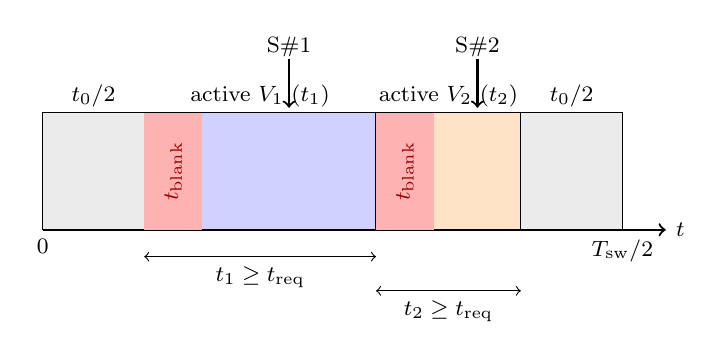
\begin{tikzpicture}[x=0.92cm,y=0.62cm]
  % time axis
  \draw[->,thick] (0,0) -- (8.6,0) node[right]{\footnotesize $t$};
  \node[below] at (0,0) {\footnotesize $0$};
  \node[below] at (8,0) {\footnotesize $\Tsw/2$};
  % segments: zero | active1 (t1) | active2 (t2) | zero
  \fill[black!8]  (0,0) rectangle (1.4,2.4);
  \fill[blue!18]  (1.4,0) rectangle (4.6,2.4);
  \fill[orange!22](4.6,0) rectangle (6.6,2.4);
  \fill[black!8]  (6.6,0) rectangle (8,2.4);
  \draw (0,0) rectangle (8,2.4);
  \draw (1.4,0)--(1.4,2.4); \draw (4.6,0)--(4.6,2.4); \draw (6.6,0)--(6.6,2.4);
  \node at (0.7,2.75){\footnotesize $t_0/2$};
  \node at (3.0,2.75){\footnotesize active $V_1$ ($t_1$)};
  \node at (5.6,2.75){\footnotesize active $V_2$ ($t_2$)};
  \node at (7.3,2.75){\footnotesize $t_0/2$};
  % blanking + treq window inside each active vector
  \fill[red!30] (1.4,0) rectangle (2.2,2.4);
  \fill[red!30] (4.6,0) rectangle (5.4,2.4);
  \node[red!60!black] at (1.8,1.2){\footnotesize\rotatebox{90}{$\tblank$}};
  \node[red!60!black] at (5.0,1.2){\footnotesize\rotatebox{90}{$\tblank$}};
  % sample instants
  \draw[->,thick] (3.4,3.5)--(3.4,2.5); \node at (3.4,3.75){\footnotesize S\#1};
  \draw[->,thick] (6.0,3.5)--(6.0,2.5); \node at (6.0,3.75){\footnotesize S\#2};
  % treq brackets
  \draw[<->] (1.4,-0.55)--(4.6,-0.55) node[midway,below]{\footnotesize $t_1\ge\treq$};
  \draw[<->] (4.6,-1.25)--(6.6,-1.25) node[midway,below]{\footnotesize $t_2\ge\treq$};
\end{tikzpicture}
\caption{Single-shunt sampling within one half-carrier. Two settled samples must fit the two active-vector plateaus $t_1$ and $t_2$; each loses $\tblank$ to switching transients and $\tmargin$ to jitter, so each plateau must satisfy $t_k\ge\treq$.}
\label{fig:timing}
\end{figure}

\subsection{Active-vector dwell times}
Let the angle within a sector be $\alpha \in [0,\pi/3]$. With definition \eqref{eq:m_def}, the two adjacent active-vector dwell times available in one half-carrier of duration $\Tsw/2$ are
\begin{equation}
t_1(\alpha) = \frac{\Tsw}{2}\,\midx\,\sin\!\Big(\frac{\pi}{3}-\alpha\Big), \quad
t_2(\alpha) = \frac{\Tsw}{2}\,\midx\,\sin(\alpha),
\label{eq:t1t2}
\end{equation}
and the local zero-vector time is
\begin{equation}
t_0(\alpha) = \frac{\Tsw}{2} - t_1(\alpha) - t_2(\alpha).
\label{eq:t0}
\end{equation}

\subsection{Regime A --- unmodified PWM: blind zones}
Without waveform modification, both samples are feasible only where
\begin{equation}
t_1(\alpha)\ge \treq \quad \text{and}\quad t_2(\alpha)\ge \treq .
\label{eq:two_windows}
\end{equation}
Because $t_2\!\to\!0$ as $\alpha\!\to\!0$ and $t_1\!\to\!0$ as $\alpha\!\to\!\pi/3$, a \emph{blind zone} of half-angle
\begin{equation}
\alpha_{\mathrm{blind}} = \arcsin\!\Big(\frac{2\treq}{\midx \Tsw}\Big)
\label{eq:alpha_blind}
\end{equation}
appears at each sector boundary (valid when $0 \le 2\treq/(\midx\Tsw) \le 1$). Higher $\midx$ lengthens the active vectors and \emph{shrinks} the blind zones, but they never vanish: at exactly the boundary one dwell is zero for any $\midx$. The widest measurable region per sector occurs at the sector center $\alpha=\pi/6$, where $t_1=t_2=\midx\Tsw/4$; requiring this best case to exist gives the existence bound
\begin{equation}
\ \midx \ge \midx_{\min,\mathrm{SS}} = \frac{4\,\treq}{\Tsw}\ 
\label{eq:m_min_ss}
\end{equation}
Operation inside the blind zones requires either PWM shaping (Regime B) or reconstruction strategies that estimate the missing sample.

\subsection{Regime B --- minimum-window enforcement: the modulation bound}
Practical drives \emph{remove} blind zones by enforcing a minimum active-vector time---measurement/minimum-vector insertion, pulse stretching, or switching-state phase shift---so both plateaus can host a sample \cite{Blaabjerg1997,Gu2011,Yan2016}. The borrowed time must come from the zero-vector reserve $t_0$ in the same half-carrier. The worst case is the sector boundary $\alpha=0$, where $t_2(0)=0$ and
\begin{equation}
t_1(0)=\frac{\Tsw}{2}\,\midx\,\frac{\sqrt{3}}{2}, \qquad
t_0(0)=\frac{\Tsw}{2}\Big(1-\midx\frac{\sqrt{3}}{2}\Big).
\label{eq:t0_boundary}
\end{equation}
To synthesize a full window $\treq$ for the collapsed vector, feasibility requires $t_0(0)\ge \treq$. Equivalently, the stretched pattern $t_1(0)+\treq$ must still fit the half-carrier, which yields the same condition. Solving for $\midx$:
\begin{equation}
\boxed{\
\midx_{\max,\mathrm{SS}}
=
\min\!\left(
1,\;
\frac{2}{\sqrt{3}}\left(1-\frac{2\,\treq}{\Tsw}\right)
\right)\ }
\label{eq:m_max_ss_main}
\end{equation}
This directly links the required sample-time budget $\treq$ to the maximum usable modulation index for \emph{full-angle} single-shunt reconstruction. Note the contrast with our dual-shunt result $\midx_{\max}=1-2\treq/\Tsw$: the single-shunt bound is tighter by the factor $2/\sqrt{3}\approx1.155$ acting on a quantity reduced by the zero-vector demand, reflecting the cost of synthesizing two windows from one channel.

\subsection{From modulation index to maximum duty cycle}
Taking the sinusoidal-reference envelope consistent with linear SVM, the per-phase duty is
\begin{equation}
\dc_k = \tfrac{1}{2} + \tfrac{\midx}{2}\sin(\theta+\phi_k),\quad \phi_k\in\{0,\mp 2\pi/3\},
\end{equation}
so the maximum duty over electrical angle is $\dc_{\max} = (1+\midx)/2$, and combining with \eqref{eq:m_max_ss_main},
\begin{equation}
\boxed{\
\dc_{\max,\mathrm{SS}} = \frac{1+\midx_{\max,\mathrm{SS}}}{2}.\ }
\label{eq:dmax_ss}
\end{equation}

% -------------------- Section VI --------------------
\section{Design Charts and a Worked Example}
\subsection{Worked example}
We anchor the budget in hardware. Measurements on a DRV8305-based low-side chain with a $65~\Omega/2200~\mathrm{pF}$ input filter (Figs.~\ref{fig:settle}--\ref{fig:xtalk}) give op-amp/PGA settling $\tacq\approx0.8~\mu\mathrm{s}$ and switching-crosstalk blanking $\tblank\approx0.1~\mu\mathrm{s}$; with $\tmargin=0.1~\mu\mathrm{s}$ this is $\treq\approx1.0~\mu\mathrm{s}$. From \eqref{eq:m_max_ss_main}, a typical $f_{sw}=20~\mathrm{kHz}$ ($\Tsw=50~\mu\mathrm{s}$) imposes no modulation limit ($\midx_{\max,\mathrm{SS}}=1$); the budget only bites at high carriers---$f_{sw}=100~\mathrm{kHz}$ gives $\midx_{\max,\mathrm{SS}}=\tfrac{2}{\sqrt{3}}(1-0.2)\approx0.92$ and $\dc_{\max,\mathrm{SS}}\approx0.96$. The companion web calculator \cite{Wendler_calc_2026} (Fig.~\ref{fig:calc}) reproduces these curves, the blind-zone map \eqref{eq:alpha_blind}, and the SVM duty waveforms for any budget.

\begin{figure}[t]
    \centering
    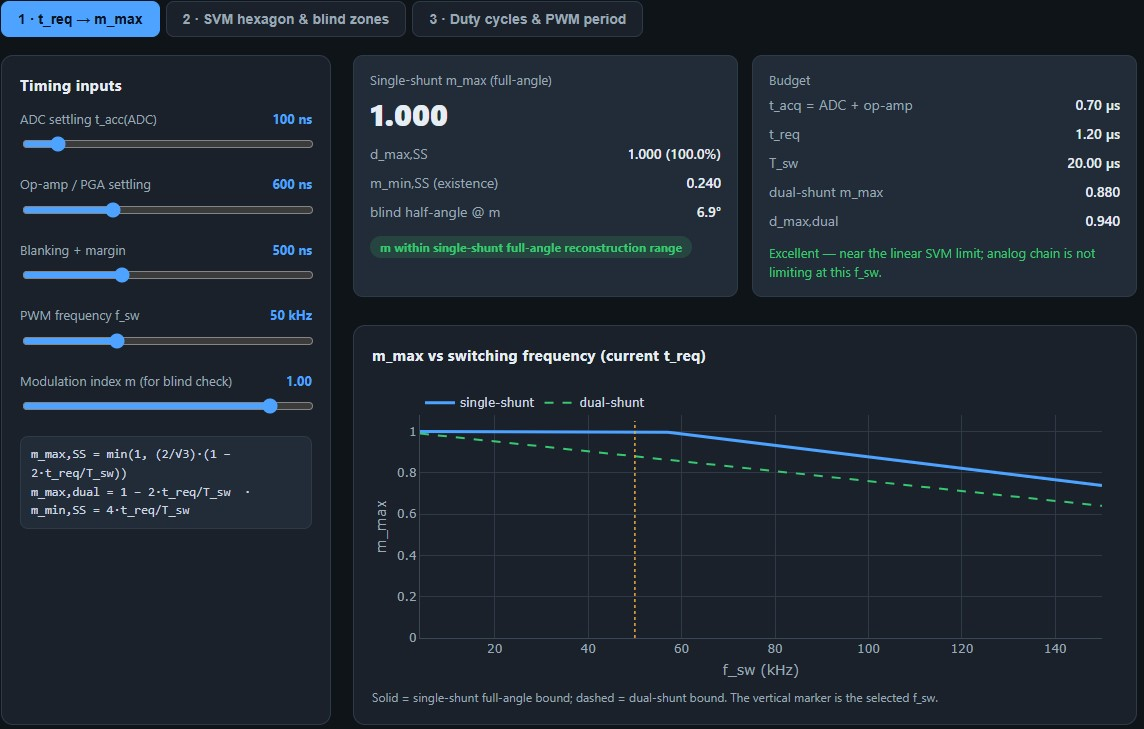
\includegraphics[width=\linewidth]{Drawings/ShuntCurrentSensingCalculator.jpg}
    \caption{Interactive companion calculator \cite{Wendler_calc_2026}: the analog timing budget $\treq=\tacq+\tblank+\tmargin$ and $f_{sw}$ map to the single-shunt modulation ceiling $\midx_{\max,\mathrm{SS}}$ from \eqref{eq:m_max_ss_main}, with the dual-shunt bound shown for comparison. The sweep panel plots $\midx_{\max,\mathrm{SS}}$ versus $f_{sw}$, the vertical marker indicating the selected frequency.}
    \label{fig:calc}
\end{figure}

\subsection{Sensitivity to switching frequency}
Table~\ref{tab:mmax} evaluates \eqref{eq:m_max_ss_main} across $f_{sw}$ for the measured budget $\treq\approx1.0~\mu$s. The ceiling stays at the linear limit through typical carriers and only collapses at high $f_{sw}$---the central design tension: higher $f_{sw}$ reduces current ripple and audible noise but shrinks the single-shunt window.

\begin{table}[t]
\caption{Single-shunt limits from \eqref{eq:m_max_ss_main} vs.\ $f_{sw}$ for the measured budget $\treq\approx1.0~\mu$s}
\label{tab:mmax}
\centering
\begin{tabular}{@{}lcc@{}}
\toprule
$f_{sw}$ & $\midx_{\max,\mathrm{SS}}$ & $\dc_{\max,\mathrm{SS}}$\\
\midrule
$20$~kHz  & $1.00$ & $1.00$\\
$50$~kHz  & $1.00$ & $1.00$\\
$100$~kHz & $0.92$ & $0.96$\\
$150$~kHz & $0.81$ & $0.90$\\
\bottomrule
\end{tabular}
\end{table}

\noindent The ENOB needed to meet an application-level RMS angle-error target $\epsilon_\theta$ follows the budget derived in the companion dual-shunt analysis; here it enters only as the floor that makes \eqref{eq:window}--\eqref{eq:treq_def} worth satisfying \cite{wendler_enhancing_2025}.

% -------------------- Section VII --------------------
\section{Signal Chain and Mitigation}
\subsection{Where the budget comes from: measured settling and blanking}
The acquisition budget is dominated by the analog signal chain, not the ADC core. An op-amp/PGA must recover from the large common-mode step at each switching edge before its output tracks the shunt voltage; this recovery plus the ADC input-RC sets $\tacq$ \cite{Kester2005,TI_SLAAE96A_2023}. Fig.~\ref{fig:settle} shows this on a DRV8305-based low-side chain with a $65~\Omega/2200~\mathrm{pF}$ filter: after the MOSFET node switches, the amplified phase-current channels settle in $\tacq\approx0.8~\mu\mathrm{s}$. Fig.~\ref{fig:xtalk} shows the complementary effect---switching noise from one leg coupling into another phase's channel---which sets a blanking interval $\tblank\approx0.1~\mu\mathrm{s}$ before a sample is trustworthy. These fix the measured budget $\treq\approx1.0~\mu\mathrm{s}$ used above. Faster settling (higher gain-bandwidth, lower CM-step via Kelvin sensing and layout) raises $\midx_{\max,\mathrm{SS}}$ through \eqref{eq:m_max_ss_main}; since integrated front ends on advanced MCU nodes trade settling for area and cost, the single-shunt ceiling is increasingly an analog-IP and process question.

\begin{figure}[t]
\centering
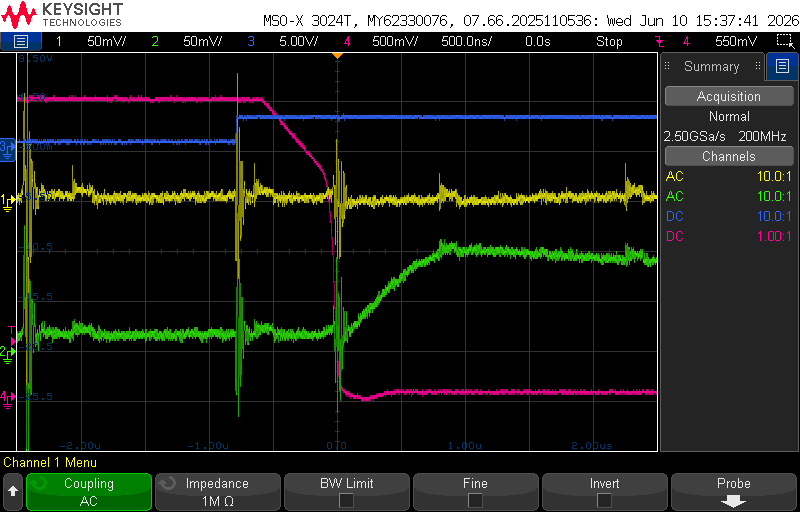
\includegraphics[width=\linewidth]{Drawings/PhaseSwitchOnCurrent_noise.png}
\caption{Measured op-amp/PGA settling (Keysight MSO-X 3024T, $500~\mathrm{ns/div}$) on a DRV8305 low-side chain with a $65~\Omega/2200~\mathrm{pF}$ filter. Blue: PWM logic; purple: MOSFET switch-node; yellow and green: the two amplified phase-current channels. After the switching edge the current channels need $\tacq\approx0.8~\mu\mathrm{s}$ to settle.}
\label{fig:settle}
\end{figure}

\begin{figure}[t]
\centering
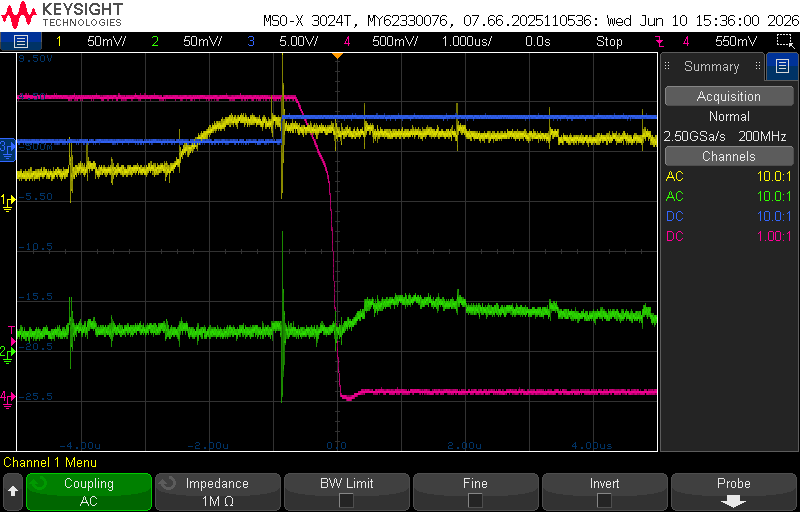
\includegraphics[width=\linewidth]{Drawings/SwitchingNoiseOnOtherphase.png}
\caption{Measured switching-noise crosstalk ($1~\mu\mathrm{s/div}$, same channels as Fig.~\ref{fig:settle}): a leg's switching event couples a short burst into another phase's current channel, defining a blanking time $\tblank\approx0.1~\mu\mathrm{s}$.}
\label{fig:xtalk}
\end{figure}

\subsection{Mitigation strategies and their cost}
When the required operating point falls inside a blind zone, the standard remedies trade either voltage headroom or spectral quality:
\begin{itemize}
\item \textbf{Minimum/measurement-vector insertion} guarantees $t_k\ge\treq$ by stretching active vectors, consuming zero-vector dwell and lowering $\midx_{\max,\mathrm{SS}}$ as in \eqref{eq:m_max_ss_main} \cite{Blaabjerg1997}.
\item \textbf{Switching-state phase shift} targets the specific blind case where two legs carry (nearly) equal duty, so the active-vector window between their coincident edges collapses (e.g.\ $t_1\!\to\!0$ when $d_a\!\approx\!d_b$). Instead of lengthening a vector, it \emph{time-shifts} one leg's pulse within the carrier period---separating the otherwise simultaneous edges to open a measurable window while leaving each leg's on-time, and hence the volt-second average, unchanged \cite{Gu2011}. Because the duty is preserved, it avoids the voltage/modulation penalty of stretching; its reach is bounded only by the zero-vector room available to shift into, so it \emph{relaxes} rather than removes the limit \eqref{eq:m_max_ss_main} as $t_0\!\to\!0$ near full modulation.
\item \textbf{Reconstruction/estimation in blind zones}---hold-last-value, model-based prediction, or sampling across both half-carriers---avoids PWM shaping at the cost of estimator complexity and error \cite{Yan2016}.
\end{itemize}
All of these are downstream of the same lever: a smaller $\treq$ enlarges the natural windows and reduces how aggressively any strategy must intervene.

% -------------------- Section VIII --------------------
\section{Engineering Takeaways}
\begin{itemize}
\item \textbf{Specify acquisition time, not MSPS.} For single-shunt sensing the binding constraint is settling within SVM plateaus; conversion speed matters only insofar as two samples share one channel.
\item \textbf{Single-shunt carries a modulation price tag.} Full-angle reconstruction obeys \eqref{eq:m_max_ss_main}; faster settling buys modulation and duty headroom one-for-one.
\item \textbf{High $f_{sw}$ and single-shunt fight each other.} The window shrinks linearly with $\Tsw$, so the modulation ceiling falls sharply above $\sim$50--100~kHz for realistic analog chains.
\item \textbf{The analog front end---and its silicon node---is the real limit.} Integrated PGAs ease cost but their settling sets $\treq$; in-line sensing remains the timing-easiest option when cost and isolation permit.
\end{itemize}

% -------------------- Conclusion --------------------
\section{Conclusion}
Single-shunt current sensing converts PWM geometry into an ADC requirement: two settled samples must fit two active-vector plateaus. Grouping analog settling, blanking, and trigger margin into $\treq$, we described the unmodified-PWM blind zones and derived a compact modulation-headroom limit for full-angle reconstruction under center-aligned SVM,
\begin{equation}
\midx_{\max,\mathrm{SS}}=\min\!\left(1,\frac{2}{\sqrt{3}}\left(1-\frac{2\treq}{\Tsw}\right)\right)
\qquad
\label{eq:conclusion_1}
\end{equation}
\begin{equation}
\dc_{\max,\mathrm{SS}}=\frac{1+\midx_{\max,\mathrm{SS}}}{2}
\label{eq:conclusion_2}
\end{equation}
\eqref{eq:conclusion_1}, \eqref{eq:conclusion_2} equations connect ADC acquisition-time reality to voltage utilization in single-shunt PMSM FOC and give an immediate rule for choosing $f_{sw}$, analog front-end settling, and PWM-shaping strategy. Future work will validate $\treq$ on hardware under PWM-induced transients and quantify the residual angle error of blind-zone estimation against the efficiency targets set by the sensorless budget.

% -------------------- References --------------------
\bibliographystyle{IEEEtran}
\bibliography{references}

\end{document}
